% !TEX root =../thesis.tex
\chapter{Linear interpolation in N-Dimensions}
\label{chap:ndinterpolation}

\lettrine[lines=4]{I}{nterpolation} is one of the most common operations in astronomy. Irregardless if one needs to resample spectra on a different wavelength grid to co-add them, projecting images to align them or interpolating physical quantities in N-dimensional fluid dynamics simulation, interpolation plays a central role.
Interpolation can be described as a special case of curve fitting which requires the function to go through all points. 

In one dimension interpolation is relatively easy and there exist multiple methods. The simplest method is nearest-neighbour interpolation in which the interpolation picks the closest neighbour point to the point to be interpolated. 

Linear interpolation is one of the most common methods of interpolation. The two neighbouring points of the point to be interpolated are found and using their slope and offset the value is interpolated.

There exist more complex interpolation methods like splines that employ polynomials of n-th degree whose first and second derivation need to be the same at the data points. 

Where there exist many methods for interpolation in one dimensional space, the number of options decreases rapidly with the number of dimensions increasing. 
Although the number of viable options is decreasing there exist still a number of methods for n-dimensional interpolation. We will focus on the implementation of linear interpolation in N-dimensions, although there are other options like nearest neighbour interpolation and Radial basis function.

For our linear interpolation we have opted to use \deltri\ as a interpolation method.

The interpolation using \deltri\ employs multiple steps to arrive at an  interpolation.

First a delauney triangulation is performed on the existing grid. As a next step we need to find the simplex that contains the point to be interpolated. 
Finally we will use the barycentric coordinate system of the simplex to perform the actual interpolation.






\section{Delauney triangulation}
\label{sec:delauney_tri}
A triangulation describes the process of connecting all points in a set with straight lines without any two lines crossing (see Figure \ref{fig:delauney_example}). It is obvious that there many ways for a set to to be triangulated. All triangulations however have the same outer boundary called the convex hull. One special kind of triangulation is the \deltri. The \deltri\ can be defined a various abstract ways and has intriguing properties.

\begin{figure}[htbp] %  figure placement: here, top, bottom, or page
   \centering
   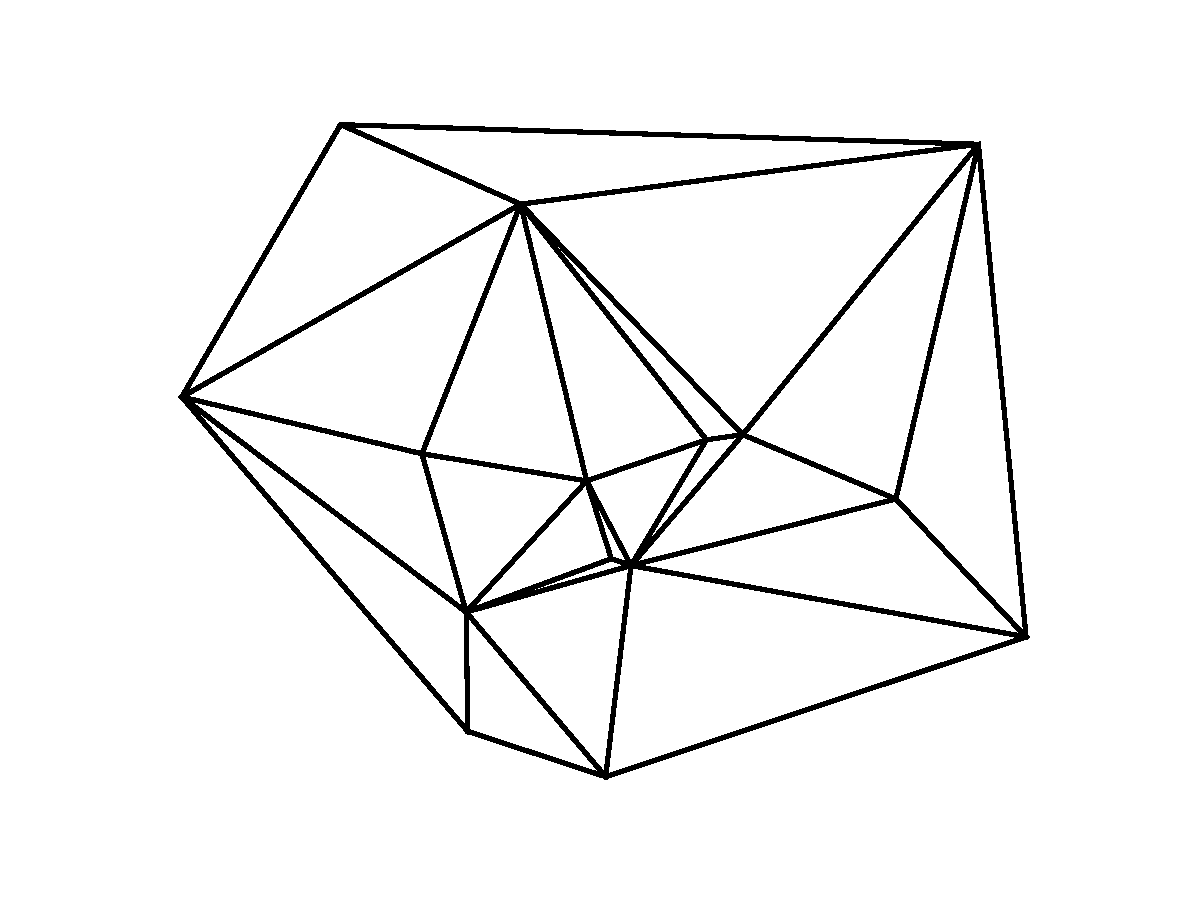
\includegraphics[width=\textwidth]{chapter_ndinterp/plots/simple_delauney.pdf} 
   \caption{The delauney triangulation of 20 points is shown above}
   \label{fig:delauney_example}
\end{figure}


One such defintion is that the circum-circle of each triangle must only contain three points. Figure \ref{fig:delauney_allowed}, a simple two dimensional example, shows one \textit{legal} triangulation and one \textit{illegal} triangulation. One can see in the \textit{illegal} triangulation that the circum-circles of both triangles contain more than tree points. By doing a simple "\textit{edge-flip}" one arrives at the delauney triangulation. In addition this ensures that the triangulation gives the largest minimum angle for both triangles. 
There

\begin{figure}[htbp] %  figure placement: here, top, bottom, or page
   \centering
   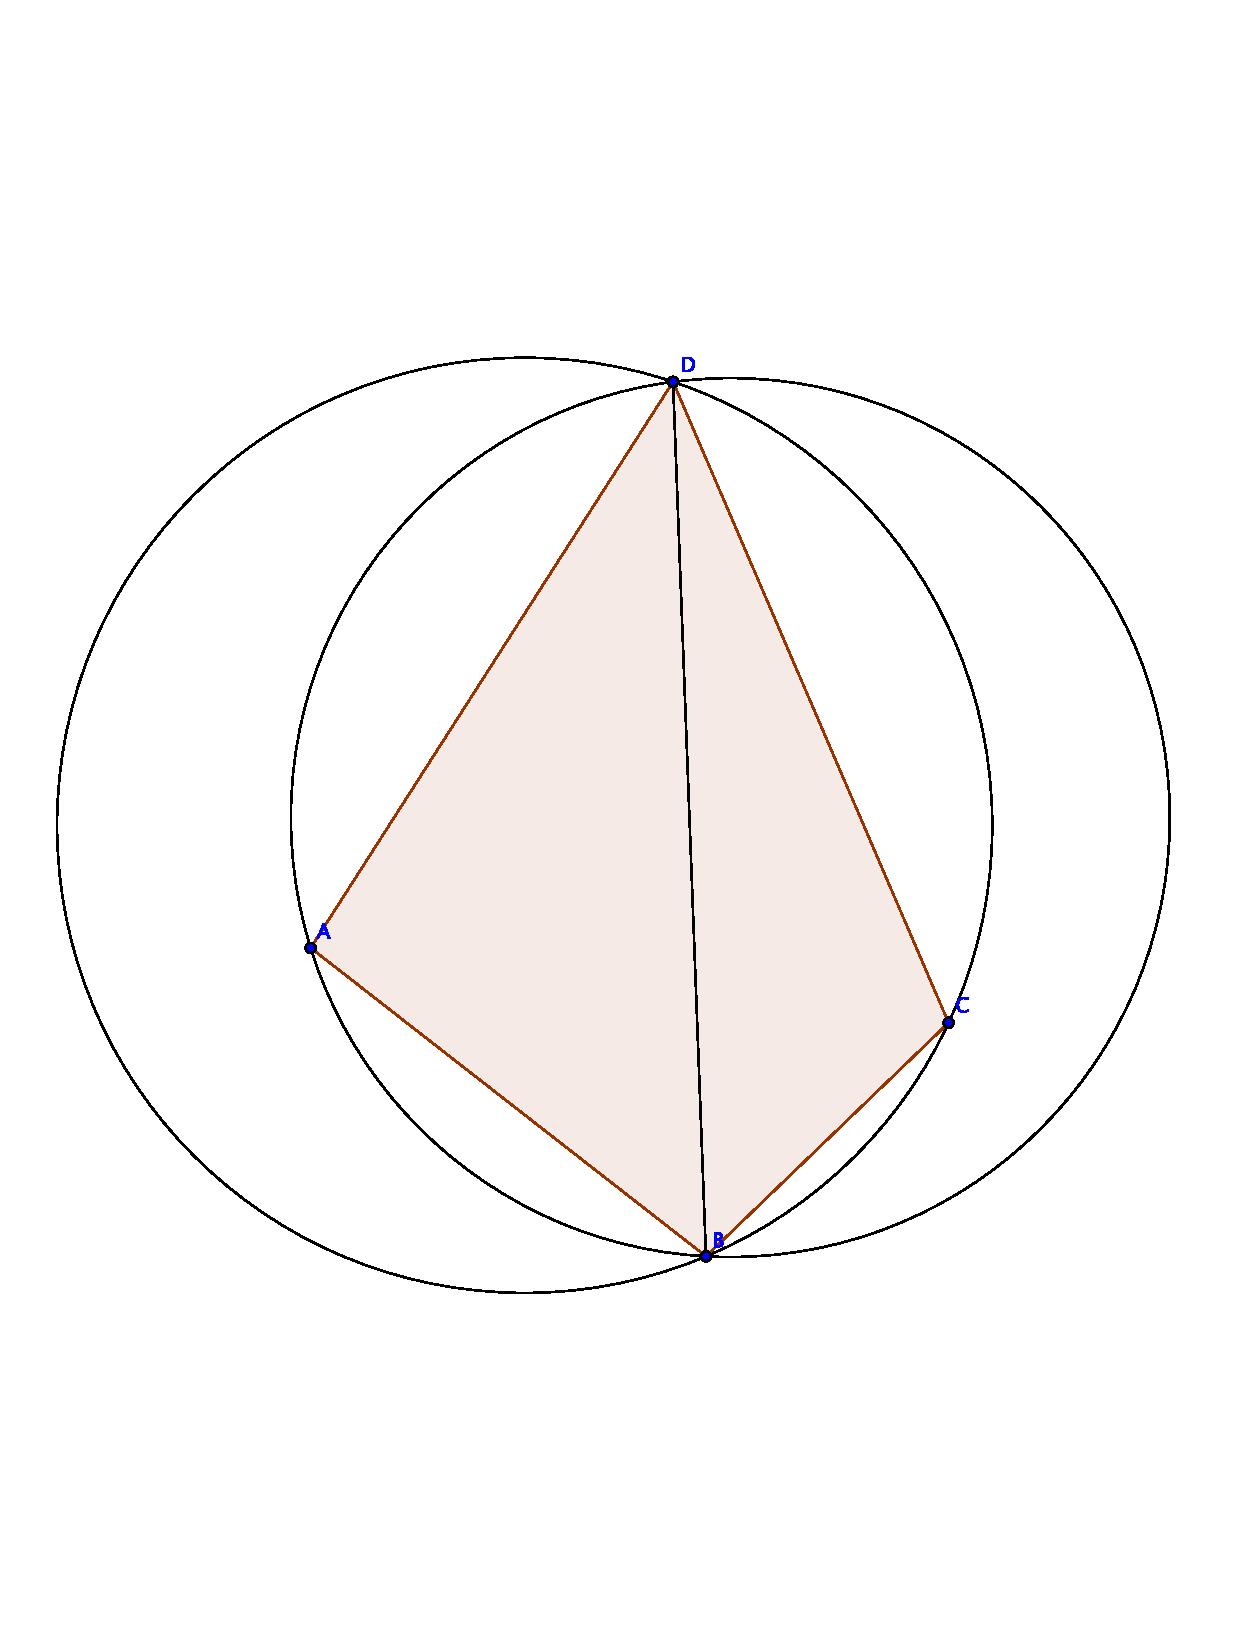
\includegraphics[width=.45\textwidth]{chapter_ndinterp/plots/illegal_triangulation.pdf} 
   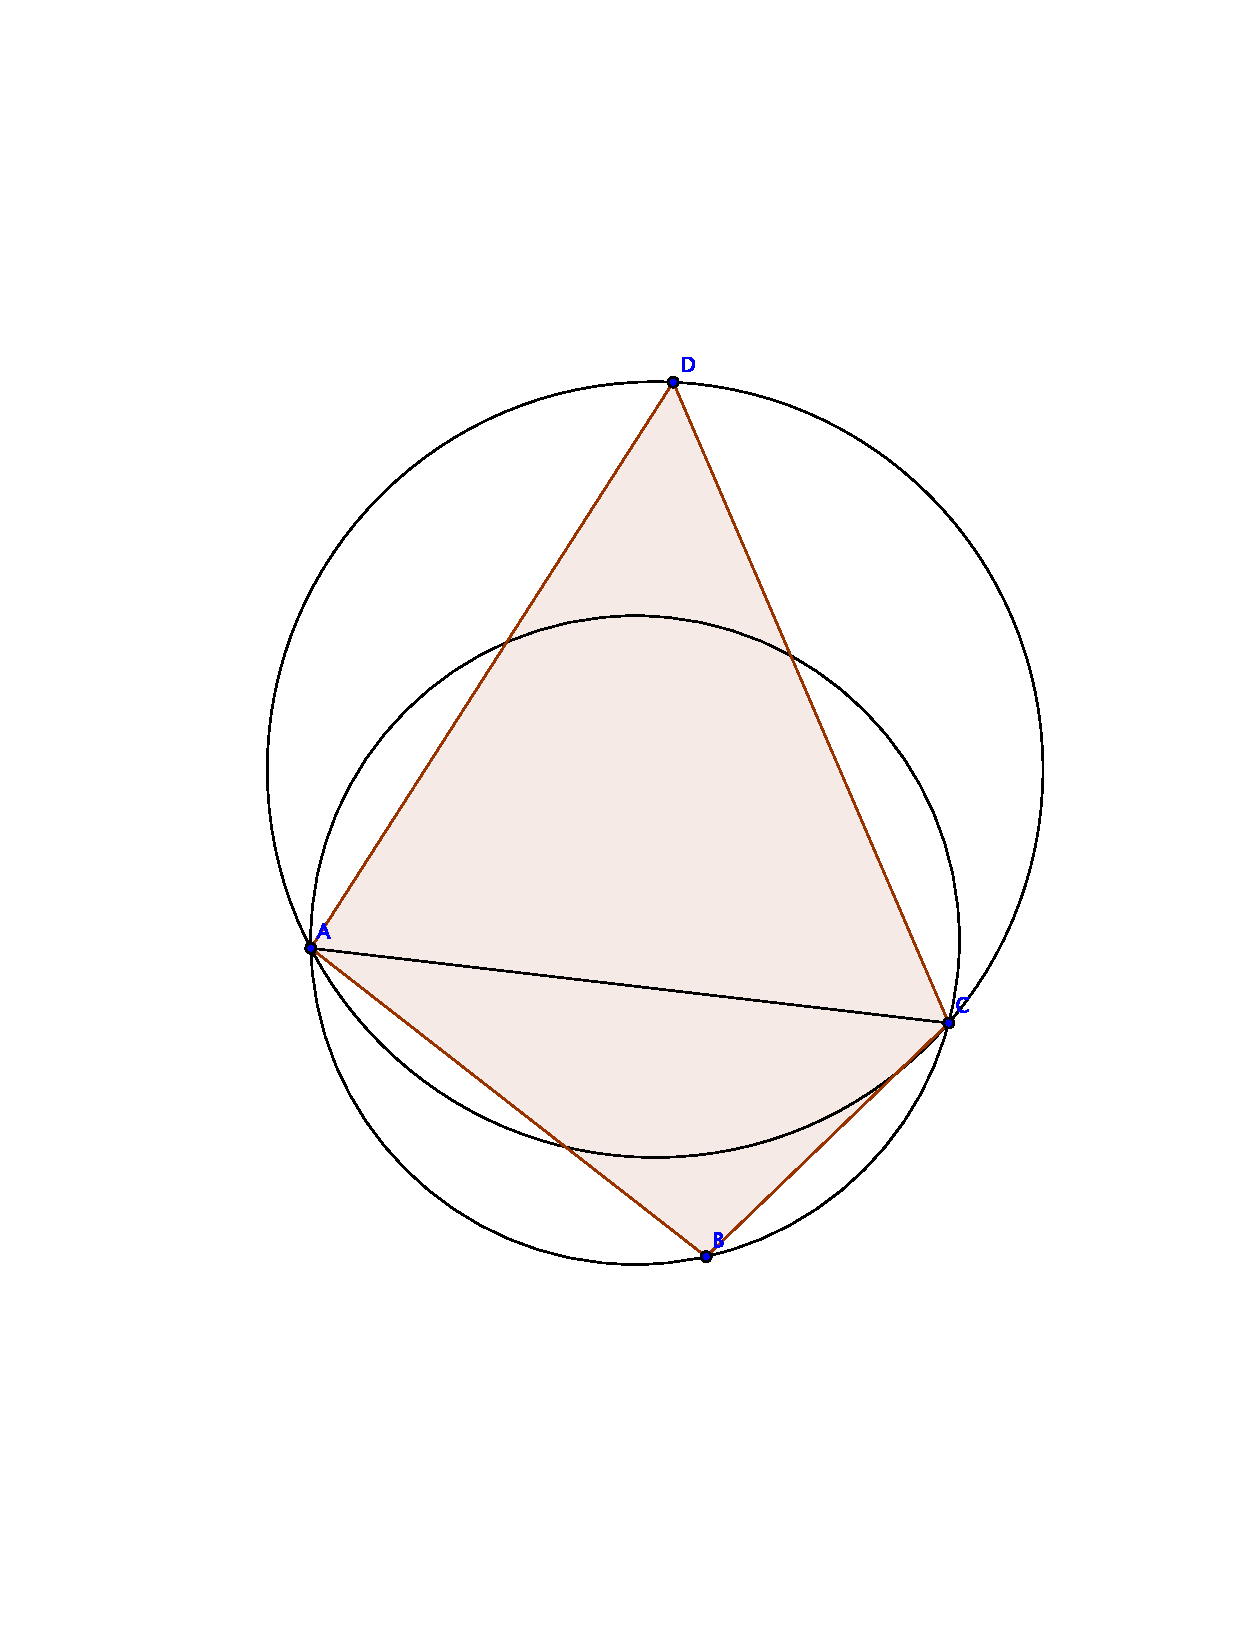
\includegraphics[width=.45\textwidth]{chapter_ndinterp/plots/edge_flip.pdf} 
   \caption{The left figure shows an "\textit{illegal}" triangulation of the 4 points. Both circles include all the points. With a so called edge flip one can arrive at a "\textit{legal}" triangulation}
   \label{fig:delauney_allowed}
\end{figure}
\deltri\ and convex hulls have a very interesting relation. It is possible construct the \deltri\ in n dimensions from a convex hull of the points projected on paraboloid in n+1 dimensions.
Figure \ref{fig:delauney_projection} shows an example of a \deltri\ in two dimensions constructed from the convex hull in three dimensions. To project the points onto the paraboloid one just square sums the coordinates n dimensions and uses this as the coordinate for the point in n+1 dimensions. 

\begin{figure}[htbp] %  figure placement: here, top, bottom, or page
   \centering
   \includegraphics[width=0.49\textwidth]{chapter_ndinterp/plots/delauney_project_left.pdf} 
   \hspace{-1.5cm}
   \includegraphics[width=0.49\textwidth]{chapter_ndinterp/plots/delauney_project_right.pdf} 
   \caption{Stereogram \citep{Vogt11} of the projection of the convex hull in three dimensions to form the delauney triangulation in two dimensions}
   \label{fig:delauney_projection}
\end{figure}

\section{Convex Hull}

In section \ref{sec:delauney_tri} we have described the relation between the convex hull  and the \deltri. There are multiple ways to construct the convex hull for N points, we will limit ourselves to the description of the Quickhull algorithm. Similar to the Quicksort algorithm it follows the divide and conquer method. 


\begin{figure}[htbp] %  figure placement: here, top, bottom, or page
   \centering%
   \subfloat[Twenty points for which we are trying to find the convex hull]{%
%   \missingfigure[figwidth=0.4\textwidth]{Test}%
   \includegraphics[width=0.4\textwidth]{chapter_ndinterp/plots/qhull_1.pdf}%
   \label{fig:qhull_1}%
 }\quad%
 \subfloat[We find the points with the lowest and highest x-value and connect them with a line]{
%   \missingfigure[figwidth=0.4\textwidth]{Test}%
   \includegraphics[width=0.4\textwidth]{chapter_ndinterp/plots/qhull_2.pdf}%
   \label{fig:qhull_2}%
 }\\%
 \subfloat[Continuing with the points on the left (same process happens recursively on the right) we find the point furthest away from the line. We then draw two more lines and build a triangle. The points inside of the triangle are not part of the convex hull and are discarded. We will repeat the current step with the two new lines of the triangle. ]{%
 %  \missingfigure[figwidth=0.4\textwidth]{Test}%
   \includegraphics[width=0.4\textwidth]{chapter_ndinterp/plots/qhull_3.pdf}%
   \label{fig:qhull_3}%
 }\qquad%
 \subfloat[We have found points of the convex hull once we can't build a new triangle anymore.]{%
%   \missingfigure[figwidth=0.4\textwidth]{Test}%
   \includegraphics[width=0.4\textwidth]{chapter_ndinterp/plots/qhull_final.pdf}%
   \label{fig:qhull_4}%
 }\quad%
   \caption{Building of a convex hull. }%
   \label{fig:example}%
\end{figure}%

As an initial input we have N data points. Although this method works in n-dimensions, we will show an example in two dimensions.
The first operation is finding the two extreme points in the horizontal axis, which are guaranteed to be part of the convex hull. 
We connect these two extreme points thus creating a division between the left and right point set. Now the divide and conquer method begins. We will only describe what happens to the left side, but imply that the same steps are taken on the right side. 
We find the point furthest away from the dividing line and add it. This forms a triangle with all points inside the triangle not belonging to the convex hull and thus we exclude them. The triangle again divides the remaining points into two sets, one left of the triangle and one right which are again iterated over recursively. 

The method is repeated until each subset only contains the start and end point of the dividing line. 
We have created the convex hull, which if projected to a $d - 1$-dimensional space provides the \deltri\ of the projected points.



\section{Barycentric coordinates system}

The actual interpolation transforms the interpolant's coordinate into the barycentric coordinates of the containing triangle.

One can construct the barycenter of a triangle by drawing lines from each point to the midpoint of the opposing side (see Figure \ref{fig:tri_barycenter}). 


\begin{figure}[htbp] %  figure placement: here, top, bottom, or page
   \centering
   \includegraphics[width=0.7\textwidth]{chapter_ndinterp/plots/barycenter.pdf}
   \caption{The triangle and its barycenter marked by the intersection of lines. }
   \label{fig:tri_barycenter}
\end{figure}


The coordinates of the barycenter M can simply be expressed by,
\[
\vec{M} = \frac{1}{3} (\vec{A} + \vec{B} + \vec{C}).
\]

Not only the barycenter can be expressed by the vectors of $\vec{A}$, $\vec{B}$ and $\vec{C}$ but every point p inside the triangle can be expressed by,
\[
\vec{p} = \alpha\vec{A} + \beta\vec{B} + \gamma\vec{C},
\]
where,
\[
\alpha + \beta + \gamma = 1
\]
. $\alpha$, $\beta$ and $\gamma$ are called the barycentric coordinates. If the point p lies within the triangle all barycentric coordinates are positive. 

\section{Triangle Finding and Interpolation}

To calculate the interpolation using barycentric coordinates we need to find the triangle that contains the interpolant. We use a method called directed walk (priv. comm. Pauli Virtanen). We choose a random starting triangle and calculate the barycentric coordinates for the interpolant and test if they are larger than 0. If all of them are larger than 0 we have found the containing Triangle. 
If the n-th (0,1 or 2 for two dimensions) barycentric coordinate is negative we jump to the neighbouring triangle which is opposite the n-th point. This is iterated until the containing triangle is found or the next jump would lead outside the convex hull. For the latter the point is outside of grid and can not be interpolated.

Once we find the triangle that contains the point p and we know the barycentric coordinates we can simply interpolate the function at the point by,
\[
f(\vec{p})=\alpha f(\vec{A}) + \beta f(\vec{B}) + \gamma f(\vec{C})
\]
where  $\vec{A}$, $\vec{B}$ and $\vec{C}$ are the points of the triangle. 


\section{Conclusion}

We have described the method of linear interpolation using delauney triangulation in two dimensions, but the method is extensible to N-dimensions. The triangles (3-simplex) become n-simplices in n-dimensions (e.g. Tetrahedron in 3 dimensions). The method, however, is very similar for higher dimensions. 

In this work we have made extensive use of n-dimensional linear interpolation using the implementation present in scipy \citescipy (using the LinearNDInterpolator function). In this case creation of the convex-hull is performed by the QHULL implementation described in \citet{Barber96thequickhull}.

We have tested the performance of the algorithm by creating a three dimensional grid with $20\times10\times10$ gridpoints and an array of 10, 000  double values at each gridpoint. 
On a standard 2011 MacBook Pro we have measured the initial build of the interpolation grid to 256\,ms
. The interpolation for random points took on average 601\,$\mu$\,s. This technique lends it very well to explore large datasets even on moderately equipped machines. 

There are drawbacks however. We have used this technique extensively to interpolate a spectral grid in three dimension (\teff, \logg\ and \feh). When trying to extract stellar parameters from an input spectrum we calculated the $\chi^2$ for the observed spectrum against the grid. The non-differentiability at the ridges can be seen even in the $\chi^2$ space. Optimizers that employ gradient methods \citep[such as MIGRAD][]{James:1975dr} show difficulties in some regions of the search space.

In summary, the presented linear n-dimensional interpolator is a very robust and quick way to explore large parameter spaces without having to compute each single point. 

Future work will be directed to exploring other n-dimensional interpolators in the astrophysical context. 

